\subsection{Level3.1: パラメータのチューニング}
\subsubsection{最適なパラメータを探すためのアプローチ}
最適なパラメータを探すために,3つのパラメータをそれぞれを探索するスクリプトを作成した.
\begin{itemize}
	\item HIDDEN.sh :HIDDENの値を1ずつ書き換えながら平均値を出力
	\item ALPHA.sh  :引数に「ALPHAの初期値」「ALPHAの刻み値」「ALPHAの最大値」を取り,連続的に実行する.
	\item ETA.sh    :ALPHA.shと同様にETAを小刻みに変更しながら実行を行う.
\end{itemize}

\subsubsection{実行結果}
\begin{itemize}
	\item H:31
	\item E:1.4
	\item A:0.5727
\end{itemize}

\begin{table}[htb]
 \begin{center}
  \caption{階層型NNによる文字認識問題の学習に要した回数}
  \label{table:level3}
  \begin{tabular}[htb]{r|l} \hline
   シード値 & 収束した回数 \\ \hline \hline
   1000 & 83 \\ \hline
   2000 & 75 \\ \hline
   3000 & 68 \\ \hline
   4000 & 139 \\ \hline
   5000 & 46 \\ \hline
   6000 & 67 \\ \hline
   7000 & 96 \\ \hline
   8000 & 122 \\ \hline
   9000 & 113 \\ \hline
   10000 & 162 \\ \hline \hline
   10試行の平均値 & 971 \\ \hline
  \end{tabular}
 \end{center}
\end{table}

\begin{figure}[h]
 \begin{center}
  \includegraphics[width=10.0cm]{level3/data.eps}
  \caption{重みを更新する様子(平均値)}
  \label{dataplot}
 \end{center}
\end{figure} 


\subsubsection{考察}
今回の探索には「SEARCH.sh」を実行して探索したものである.このスクリプトは各パラメータを逐次変更しながら数値が減少する方向に移動し数値の増加幅がある程度を超えると次の段階へ数値を進めるものである.
